\documentclass[tikz,border=4pt]{standalone}
\usepackage{amsmath}
\usepackage{xcolor}
\usetikzlibrary{arrows.meta,positioning,calc}

\definecolor{mhblue}{HTML}{2D76B9}
\definecolor{mhgreen}{HTML}{25895B}
\definecolor{mhorange}{HTML}{C86B2A}
\definecolor{mhpurple}{HTML}{6D4EB3}
\definecolor{mhred}{HTML}{D33A41}
\definecolor{mhslate}{HTML}{607284}
\definecolor{mhsoft}{HTML}{EEF3F8}

\begin{document}
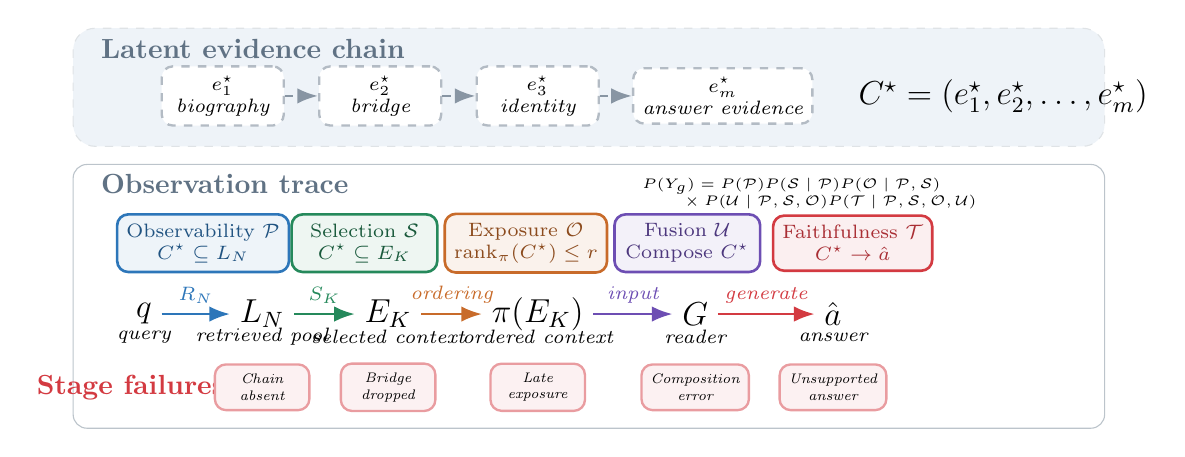
\begin{tikzpicture}[
  font=\sffamily,
  >=Latex,
  unit/.style={draw=mhslate!48, dashed, rounded corners=4pt, fill=white,
    line width=0.85pt, minimum width=1.55cm, minimum height=0.70cm,
    align=center, font=\scriptsize\itshape},
  event/.style={rounded corners=4pt, line width=0.95pt, minimum width=1.85cm,
    minimum height=0.70cm, align=center, font=\scriptsize},
  fail/.style={draw=mhred!50, fill=mhred!7, rounded corners=4pt,
    line width=0.85pt, minimum width=1.20cm, minimum height=0.58cm,
    align=center, font=\tiny\itshape},
  flow/.style={line width=1.0pt, -Latex},
  lab/.style={font=\scriptsize\itshape},
  obj/.style={font=\large}
]

\draw[draw=mhslate!20, fill=mhsoft, rounded corners=8pt, dashed]
  (0.35,3.78) rectangle (13.45,5.28);
\node[anchor=west, font=\bfseries\color{mhslate}] at (0.58,5.02)
  {Latent evidence chain};

\node[unit] (c1) at (2.25,4.42) {$e_1^\star$\\biography};
\node[unit] (c2) at (4.25,4.42) {$e_2^\star$\\bridge};
\node[unit] (c3) at (6.25,4.42) {$e_3^\star$\\identity};
\node[unit, minimum width=2.05cm] (cm) at (8.60,4.42) {$e_m^\star$\\answer evidence};
\draw[flow, dashed, mhslate!75] (c1) -- (c2);
\draw[flow, dashed, mhslate!75] (c2) -- (c3);
\draw[flow, dashed, mhslate!75] (c3) -- (cm);
\node[obj, right=0.45cm of cm] {$C^\star=(e_1^\star,e_2^\star,\ldots,e_m^\star)$};

\draw[draw=mhslate!42, rounded corners=5pt]
  (0.35,0.20) rectangle (13.45,3.55);
\node[anchor=west, font=\bfseries\color{mhslate}] at (0.58,3.30)
  {Observation trace};

\node[align=left, font=\tiny] at (9.70,3.18)
  {$P(Y_g)=P(\mathcal P)P(\mathcal S\mid\mathcal P)P(\mathcal O\mid\mathcal P,\mathcal S)$\\
   $\qquad{}\times P(\mathcal U\mid\mathcal P,\mathcal S,\mathcal O)
   P(\mathcal T\mid\mathcal P,\mathcal S,\mathcal O,\mathcal U)$};

\node[obj] (q) at (1.25,1.65) {$q$};
\node[obj] (ln) at (2.75,1.65) {$L_N$};
\node[obj] (ek) at (4.35,1.65) {$E_K$};
\node[obj] (pi) at (6.25,1.65) {$\pi(E_K)$};
\node[obj] (g) at (8.25,1.65) {$G$};
\node[obj] (ahat) at (10.00,1.65) {$\hat a$};

\draw[flow, mhblue] (q) -- node[lab, above] {$R_N$} (ln);
\draw[flow, mhgreen] (ln) -- node[lab, above] {$S_K$} (ek);
\draw[flow, mhorange] (ek) -- node[lab, above] {ordering} (pi);
\draw[flow, mhpurple] (pi) -- node[lab, above] {input} (g);
\draw[flow, mhred] (g) -- node[lab, above] {generate} (ahat);

\node[lab] at (1.25,1.36) {query};
\node[lab] at (2.75,1.36) {retrieved pool};
\node[lab] at (4.35,1.36) {selected context};
\node[lab] at (6.25,1.36) {ordered context};
\node[lab] at (8.25,1.36) {reader};
\node[lab] at (10.00,1.36) {answer};

\node[event, draw=mhblue, fill=mhblue!8, text=mhblue!70!black] at (2.00,2.55)
  {Observability $\mathcal P$\\$C^\star\subseteq L_N$};
\node[event, draw=mhgreen, fill=mhgreen!8, text=mhgreen!65!black] at (4.05,2.55)
  {Selection $\mathcal S$\\$C^\star\subseteq E_K$};
\node[event, draw=mhorange, fill=mhorange!9, text=mhorange!70!black] at (6.10,2.55)
  {Exposure $\mathcal O$\\$\operatorname{rank}_\pi(C^\star)\le r$};
\node[event, draw=mhpurple, fill=mhpurple!8, text=mhpurple!70!black] at (8.15,2.55)
  {Fusion $\mathcal U$\\Compose $C^\star$};
\node[event, draw=mhred, fill=mhred!8, text=mhred!80!black] at (10.25,2.55)
  {Faithfulness $\mathcal T$\\$C^\star\rightarrow \hat a$};

\node[font=\bfseries\color{mhred}] at (1.08,0.72) {Stage failures};
\node[fail] at (2.75,0.72) {Chain\\absent};
\node[fail] at (4.35,0.72) {Bridge\\dropped};
\node[fail] at (6.25,0.72) {Late\\exposure};
\node[fail] at (8.25,0.72) {Composition\\error};
\node[fail] at (10.00,0.72) {Unsupported\\answer};

\end{tikzpicture}
\end{document}
